%!TEX TS-program = xelatex

% Официальный шаблон презентации НИУ ВШЭ в beamer (LaTeX)
% Версия 2.0
% Язык — русский   
% Автор шаблона - Данил Фёдоровых (fedorovykh@gmail.com)

%%% Для корректной работы шаблона необходима 
%%% установка в систему бесплатного шрифта HSE Sans
%%% https://www.hse.ru/info/brandbook/#font


\documentclass[aspectratio=169]{beamer}

\usepackage{HSE-theme/beamerthemeHSE} % Подгружаем тему

%%% Работа с русским языком и шрифтами
\usepackage[english,russian]{babel}   % загружает пакет многоязыковой вёрстки
\usepackage{fontspec}      % подготавливает загрузку шрифтов Open Type, True Type и др.
\setsansfont{HSE Sans} 
\setmonofont{Courier New}
\uselanguage{russian}
\languagepath{russian}
\deftranslation[to=russian]{Theorem}{Теорема}
\deftranslation[to=russian]{Definition}{Определение}
\deftranslation[to=russian]{Definitions}{Определения}
\deftranslation[to=russian]{Corollary}{Следствие}
\deftranslation[to=russian]{Fact}{Факт}
\deftranslation[to=russian]{Example}{Пример}
\deftranslation[to=russian]{Examples}{Примеры}

%multi-row
\usepackage{multirow}
\usepackage{caption}
\usepackage{amssymb}% http://ctan.org/pkg/amssymb
\usepackage{pifont}% http://ctan.org/pkg/pifont
\usepackage{blindtext} 		% Случайный текст
\graphicspath{{images/}}  	% Папка с картинками

%%% Информация об авторе и выступлении
\title[Заголовок]{Колоризация изображений} 
%\subtitle{}
\author{Головин Вячеслав \and Саленек Иван}
%\institute{Название подразделения одну, две или три строки}
\date{\today}

\begin{document}	% Начало презентации
\renewcommand{\inserttotalframenumber}{5}   % Надо будет починить

\frame[plain]{\titlepage}	% Титульный слайд

\begin{frame}{Постановка задачи}
%\framesubtitle{}
\end{frame}

\begin{frame}{\href{https://github.com/richzhang/colorization}{Colorful Image Colorization} (2016, 2017)}
\framesubtitle{Известные результаты}
        \begin{figure}
            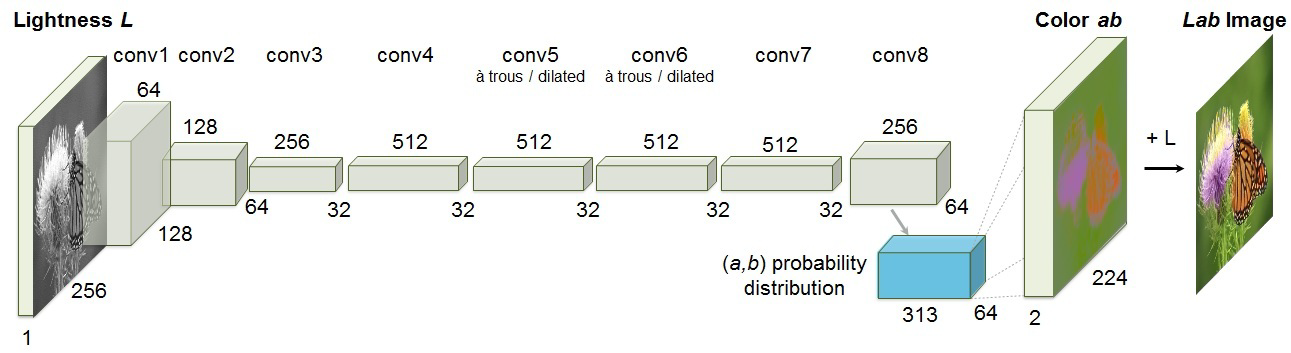
\includegraphics[width=0.6\textwidth]{eccv16.png}
            \caption*{ECCV16}
        \end{figure}

        \begin{figure}
            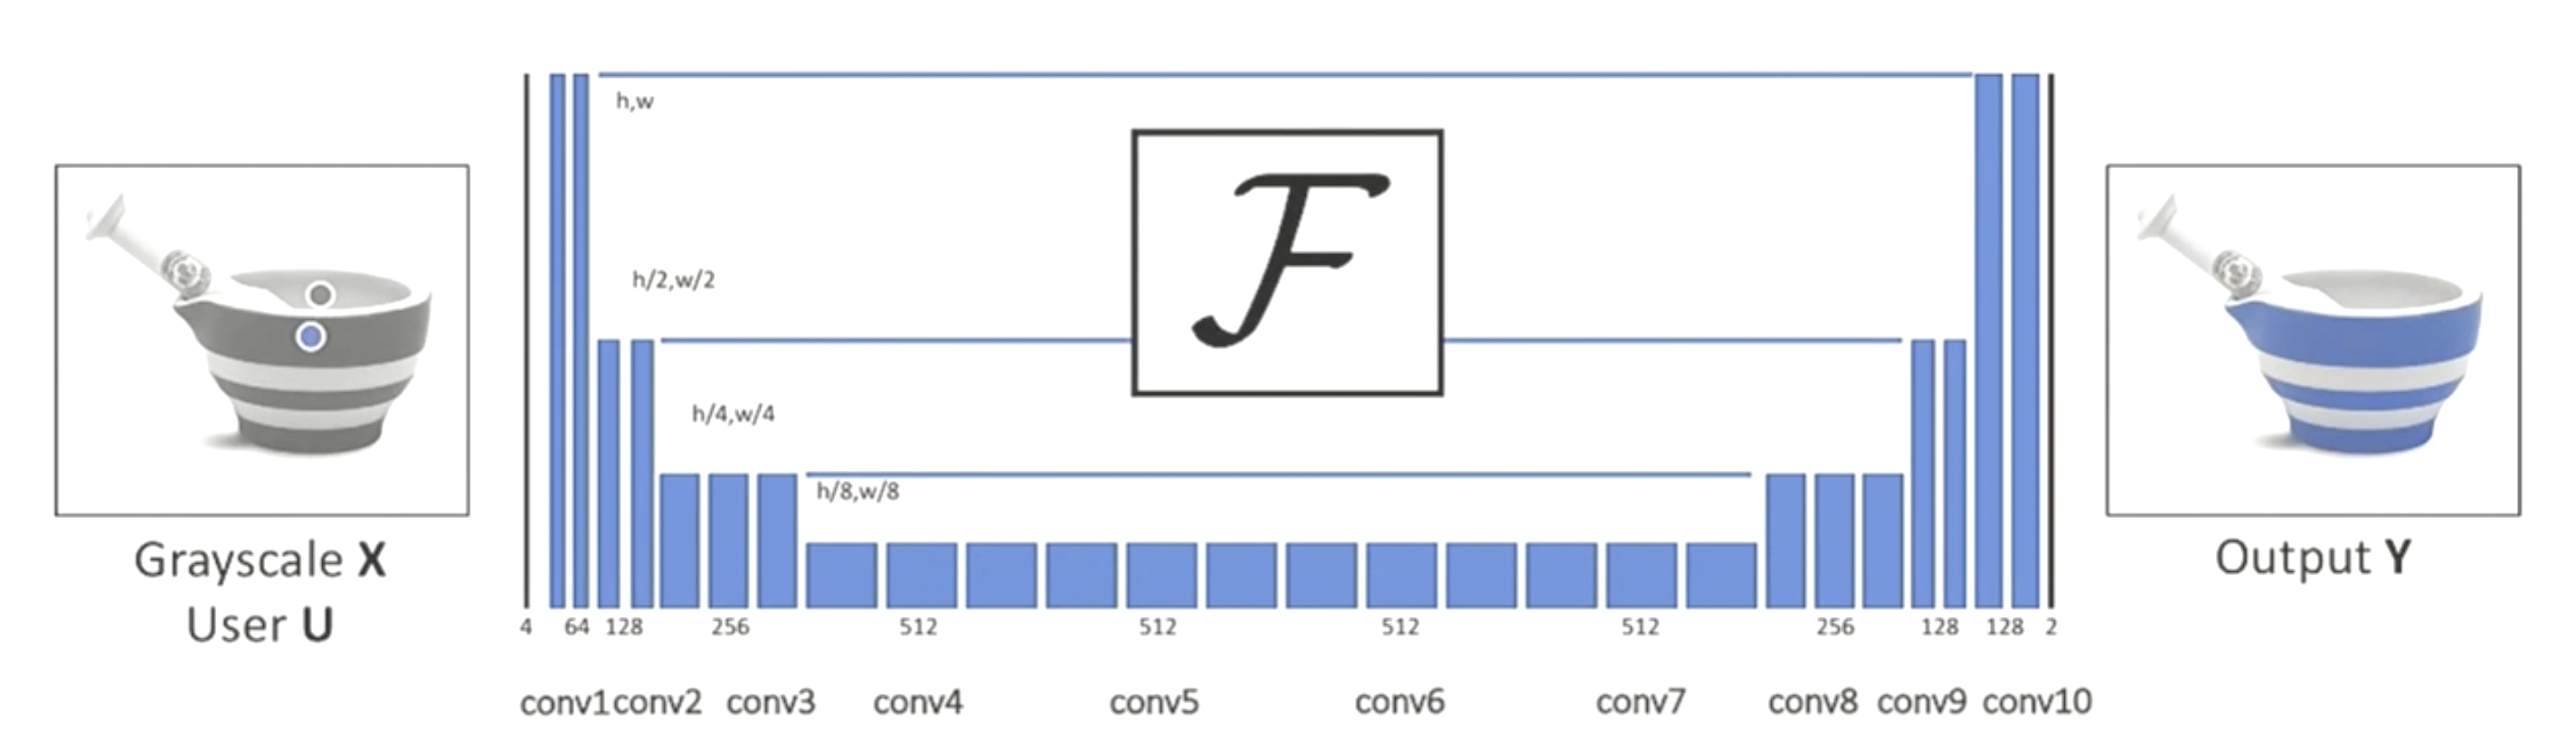
\includegraphics[width=0.6\textwidth]{siggraph17_white.png}
            \caption*{Siggraph17}
        \end{figure}
\end{frame}

\begin{frame}{\href{https://github.com/jantic/DeOldify}{DeOldify} (2018)}
    \framesubtitle{Известные результаты}

    В основе \textbf{DeOldify} лежит \textbf{GAN} архитектура. Автор использует собственный \textbf{NoGAN} подход, для обучения генератора и критика\\[3mm]
    
    Генераторам выступает \textbf{U-Net} из фреймворка \texttt{fast.ai}, позволяющего использовать предобученную сеть (н-р \textbf{ResNet}) в качестве основы для \textbf{U-Net}\\[3mm]

    \textbf{DeOldify} предлагает \textbf{2} предобученных "колорайзера":\\[3mm]
    \begin{itemize}
        \item \textbf{Artistic} -- \texttt{resnet34} в основе \textbf{U-Net} + 5 \textbf{NoGAN} итераций. \\
        $\checkmark$ Более яркие и детальные результаты \\
        \ding{55} {} Возникают артефакты
        \item \textbf{Stable} -- \texttt{resnet101} в основе \textbf{U-Net} + 3 \textbf{NoGAN} итерации. \\ 
        $\checkmark$ Лучше работает для пейзажей и портретов \\
        \ding{55} {} Более тусклые цвета
    \end{itemize}
\end{frame}

\begin{frame}{Реализованные бейзлайны}
%\framesubtitle{}

\begin{table}
    \begin{tabular}{l|c|c|c|c}
    \hline
    \multicolumn{5}{c}{Colorization Results on 1000 224x224 images}\\ 
    \hline
    \hline
    \multirow{3}{*}{Method} & \multicolumn{2}{c|}{Model} &  \multicolumn{2}{c}{Losses}\\
                            & Params & Runtime & VGG16 & MSE \\
                            & (MB) & (s) & (loss) & (loss) \\
    \hline
    CIC-ECCV16 & 129 & 250 & 0.52579 & 0.00902\\
    CIC-siggraph17 & 137 & 1232 & 0.45244 & 0.00655 \\
    \hline 
    DeOldify Stable & 874 & 4301 & 0.45699 & 0.00695\\
    DeOldify Artist & 255 & 4287 & 0.46735 & 0.00696\\


    

    \end{tabular}
\end{table}

\end{frame}

\begin{frame}{План экспериментов}
%\framesubtitle{}
\end{frame}


\end{document}